\chapter{Project Plan}

\section{Meetings}
Our goals were outlined by weekly meetings. We regularly met with Jacob Graff, our advisor throughout the development of Extend.
Jacob served as a sounding board whenever Extend's fundamental design philosophy was debated, and as a guide as we determined whether we were on track. We used any leftover time on those days to set goals for the upcoming week and pair program if time permitted.
\newline \newline
Our team also met weekly on Fridays to further discuss the progression of Extend. In the first half of the semester, the discussions were primarily philosophical, as decisions had to be made about the language grammar and behavior of certain Extend artifacts prior to development. In the second half, time was devoted to ironing out the development timeline, discussing bugs, and making compiler implementation decisions.

\section{Development Workflow}
  \begin{center}
  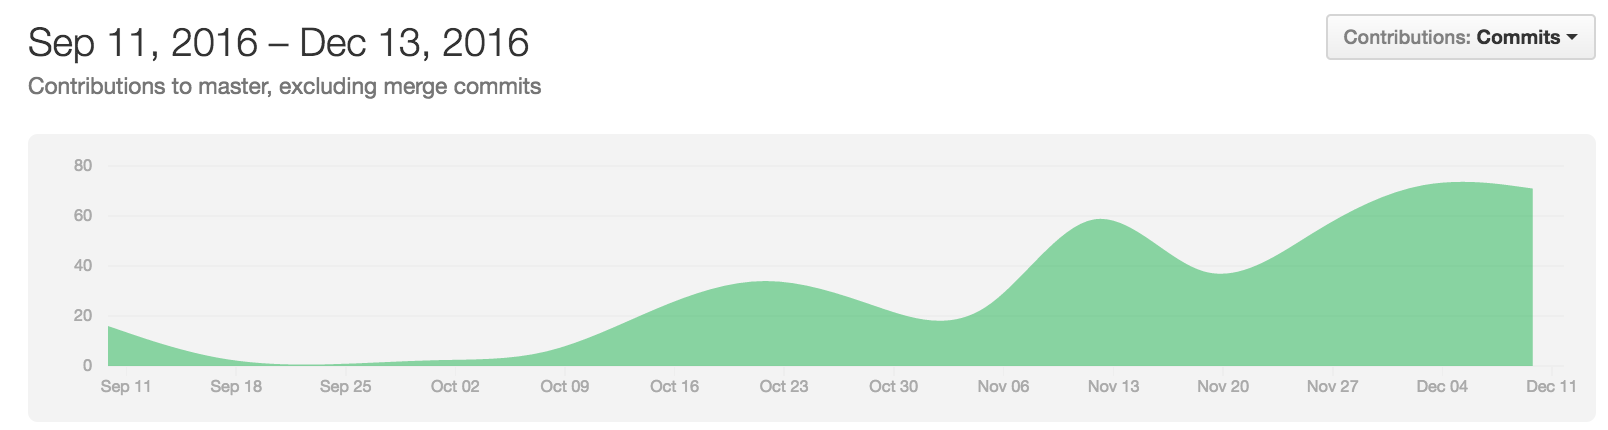
\includegraphics[width=.9\textwidth]{img/extend_git_graph.png}
  \end{center}

  \subsection{Github \& Travis CI}
  Our development and documentation were all done entirely through version control to maximize independent productivity.
  New features were introduced to the master branch through pull requests, and the team used this as a platform to peer review code to maximize code quality before such features entered production.

  \medskip \noindent
  An important aspect of development for us was continuous integration. We used Travis CI to trigger project builds on each pull request, which kept us informed regarding unexpected hiccups that sometimes arose during development. Travis CI ensured that new features were implemented with protecting the code base in mind, and provided quick visibility as to whether a new feature would break the existing build.

\section{Team Member Responsibilities}

\begin{tabular}{ | l | l | l |}\hline
  Team Member  & Responsibilities      & GitHub Profile\\ \hline
  Jared Samet & design philosophy, semantic transformations, code generation  & \underline{\href{https://github.com/oracleofnj}{oracleofnj}}\\
  Nigel Schuster & development protocol, code generation, scripting  & \underline{\href{https://github.com/Neitsch}{Neitsch}}\\
  Ishaan Kolluri & initial LRM, Final Report, regression tests, stdlib functions, scripting & \underline{\href{https://github.com/ishaankolluri}{ishaankolluri}}\\
  Kevin Ye & initial scanner, regression tests, stdlib functions & \underline{\href{https://github.com/kevinye1}{kevinye1}}\\ \hline
\end{tabular}
